\documentclass[10pt]{article}
\usepackage[letterpaper, margin=0.75in]{geometry}
\usepackage{times}
\usepackage{booktabs}
\usepackage{tabularx}
\usepackage{hyperref}
\usepackage{xcolor}
\usepackage{titlesec}
\usepackage{enumitem}
\usepackage{graphicx}
\usepackage{listings}
\usepackage{tikz}
\usepackage{seqsplit}
\usepackage{caption}
\usetikzlibrary{arrows.meta}

\definecolor{navy}{RGB}{30,39,97}
\definecolor{warn}{RGB}{153,0,0}
\definecolor{warnbg}{RGB}{255,244,229}
\definecolor{measured}{RGB}{27,94,32}
\definecolor{simulated}{RGB}{28,114,147}
\definecolor{estimated}{RGB}{191,87,0}
\definecolor{pending}{RGB}{153,0,0}
\definecolor{codebg}{RGB}{245,245,245}

% --- Compact / conference-density spacing ---
\setlength{\parskip}{3pt plus 1pt minus 1pt}
\setlength{\parindent}{0pt}
\titlespacing*{\section}{0pt}{9pt}{4pt}
\titlespacing*{\subsection}{0pt}{7pt}{3pt}
\titlespacing*{\subsubsection}{0pt}{6pt}{2pt}
\titleformat{\section}{\normalfont\large\bfseries\color{navy}}{\thesection}{0.6em}{}
\titleformat{\subsection}{\normalfont\normalsize\bfseries}{\thesubsection}{0.6em}{}
\setlist{nosep, leftmargin=1.4em}
\captionsetup{font=footnotesize, labelfont=bf, skip=4pt}
\renewcommand{\arraystretch}{0.95}

\hypersetup{colorlinks=true, linkcolor=navy, citecolor=navy, urlcolor=navy}

\lstset{
  backgroundcolor=\color{codebg},
  basicstyle=\ttfamily\scriptsize,
  breaklines=true,
  frame=single,
  rulecolor=\color{gray!40},
  columns=fullflexible,
  keepspaces=true,
  aboveskip=4pt,
  belowskip=4pt,
}

\title{\vspace{-1.2em}\textbf{One Instruction to One Megawatt}\\
\large Simulation and Measurement Methodology for Chip-to-Grid Agentic AI
Energy Behavior}
\author{Deepak Panigrahy, Aakash Tyagi \\ \small Texas A\&M University}

\date{}

\begin{document}
\maketitle
\vspace{-2.2em}

\noindent\small\textbf{Purpose.} This document has two purposes: (i) to
simulate rack-level correlation behavior from real single-node traces, and
(ii) to record every number used in the chip-to-grid chain in
Figure~\ref{fig:full}, together with the underlying queries, for
reproducibility. Companion artifacts (frozen database snapshot, raw trace
files, simulation script, full query log) are versioned alongside this
document in the project repository.
\vspace{0.2em}

\begin{figure}[h]
\centering
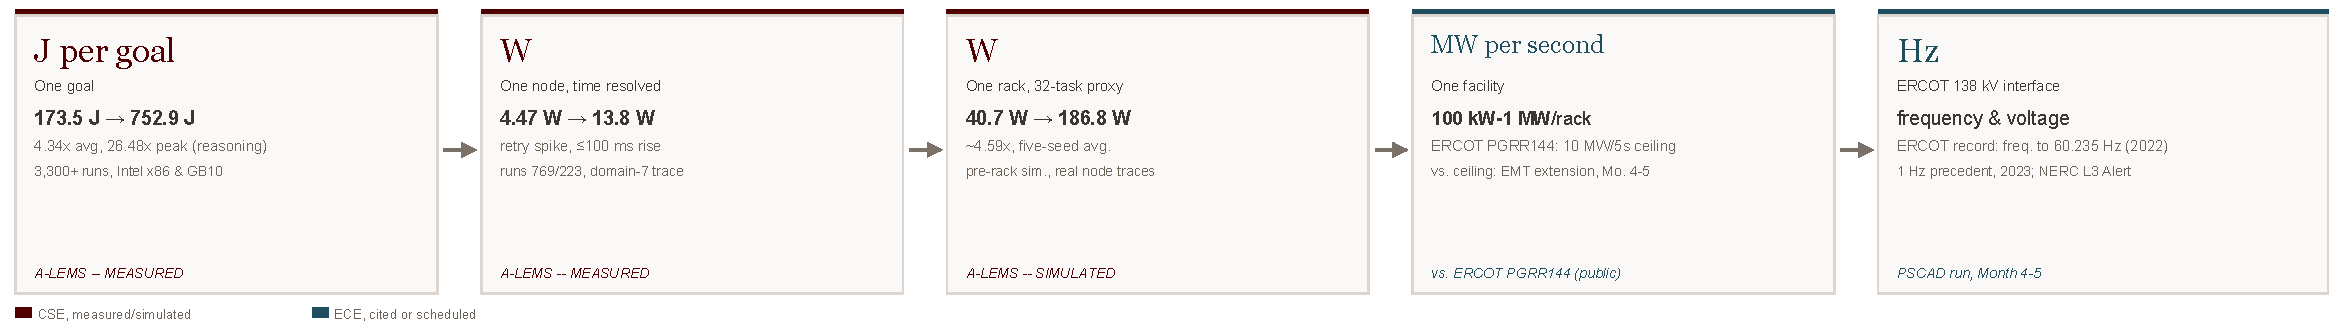
\includegraphics[width=\textwidth]{fig2/figure2_compact.pdf}
\vspace{-4pt}
\caption{Condensed view of the chip-to-grid chain. Full detail diagram and
legend in Figure~\ref{fig:full}.}
\label{fig:slim}
\end{figure}
\vspace{-4pt}
\begin{figure}[h]
\centering
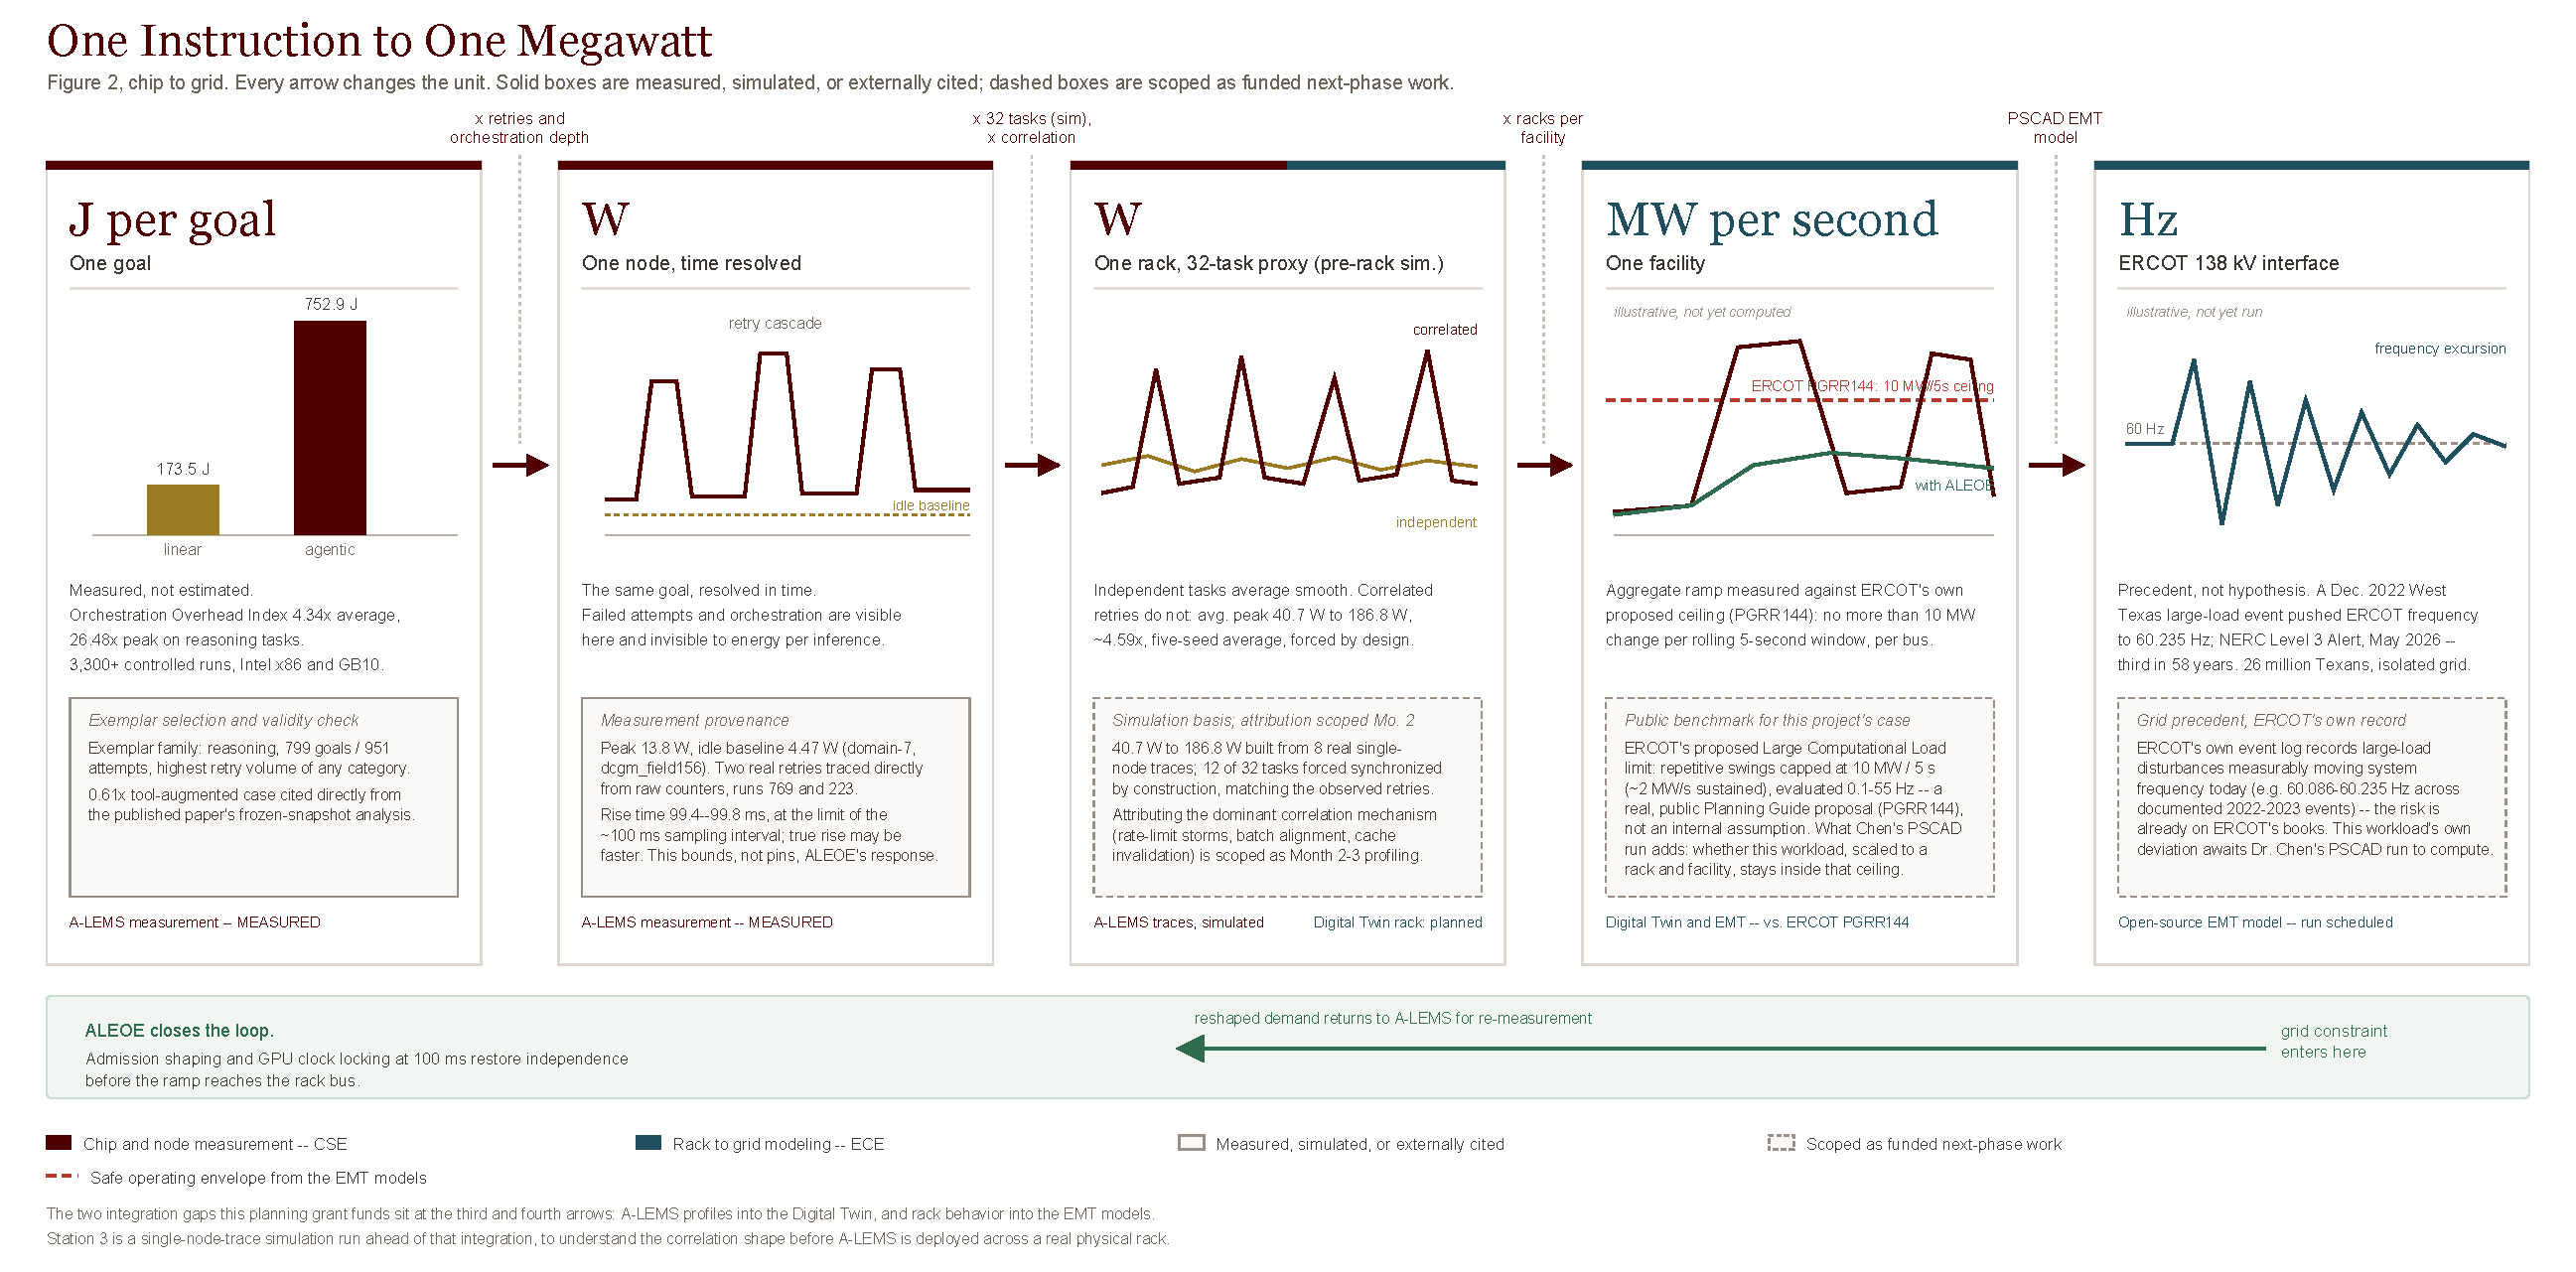
\includegraphics[width=\textwidth]{fig2/figure2_enhanced.pdf}
\vspace{-4pt}
\caption{One instruction to one megawatt: five stations tracing an agentic
AI workload's energy cost from a single chip-level goal to a grid-scale
power event. Solid-bordered boxes are measured, simulated, or externally
cited; dashed-bordered boxes are scoped as future work.}
\label{fig:full}
\end{figure}

\section{Source Data}

All measured values are drawn from a frozen snapshot of the A-LEMS
experiments database (\seqsplit{experiments\_snapshot\_figure2\_20260901.db}),
taken 2026-09-01 from the live \texttt{experiments.db} on host
\texttt{gn100-2b96}. A frozen snapshot is used rather than the live,
continuously-growing database specifically so that every number in this
document and in Figure~\ref{fig:full} remains reproducible against a fixed dataset, rather
than drifting as new runs are added.

\section{Measurement Method Finding: GPU Attribution Is Not Uniform Across Runs}
\label{sec:method-finding}

During data collection it was discovered that GPU energy in the
\texttt{runs} table is attributed by one of at least two distinct methods,
recorded in \texttt{runs.gpu\_attribution\_method}: \texttt{dcgm\_field156}
(a direct hardware counter, via NVIDIA DCGM field 156) and
\texttt{spbm\_package\_v1} (apparently derived from package-level SPBM
readings rather than a GPU-specific counter). These two methods are not
interchangeable: runs using \texttt{spbm\_package\_v1} were found to have
incomplete or entirely absent \texttt{gpu\_total\_energy\_uj} /
\texttt{gpu\_dynamic\_energy\_uj} values, and are excluded from all
Figure~\ref{fig:full} calculations. Only runs confirmed to use \texttt{dcgm\_field156}
are used as source material below.

\section{Multi-Level GPU Power Instrumentation}
\label{sec:reconciliation}

A-LEMS instruments GPU power at more than one granularity for the same run:
a direct rail-level hardware counter (domain-7, \texttt{dcgm\_field156}) and
platform-level total/dynamic energy accounting. The two report different
absolute magnitudes, as expected -- domain-7 isolates a single GPU power
rail, while the total/dynamic columns aggregate broader package-level draw.
Table~\ref{tab:reconciliation} gives both levels for two representative
runs. Figure~\ref{fig:full} uses the domain-7, above-idle-baseline reading
(Section~\ref{sec:conservative}) because it is the most directly
attributable signal to a single workload. Full-precision values are given
in Appendix~\ref{app:variance}.

\begin{table}[h]
\centering
\small
\begin{tabularx}{\textwidth}{lXXX}
\toprule
\textbf{Run ID} & \textbf{Domain-7 trace avg.\ (W)} & \textbf{Total energy / duration (W)} & \textbf{Dynamic energy / duration (W)} \\
\midrule
223 & $\approx$1--14 (idle $\approx$4.47, spike $\approx$13.8) & 61.21 & 23.50 \\
769 & $\approx$1--14 (idle $\approx$4.47, spike $\approx$13.8) & 70.78 & 5.48 \\
\bottomrule
\end{tabularx}
\vspace{-2pt}
\caption{GPU power for two representative retry runs at two instrumentation
levels: domain-7 rail power (used in Figure~\ref{fig:full}) and platform-level
total/dynamic energy accounting (used for whole-package energy and carbon
reporting elsewhere in A-LEMS). Magnitudes differ across levels because each
measures a different physical scope; the total-to-domain-7 ratio varies by
run (223: $\approx$4.4x; 769: $\approx$5.1x), consistent with per-run
differences in package-level activity outside the GPU rail itself.}
\label{tab:reconciliation}
\end{table}

\subsection{Idle baseline, separately confirmed consistent}

Unlike the total/dynamic reconciliation above, the domain-7 idle baseline
itself was verified as internally consistent. Computing
\texttt{gpu\_baseline\_energy\_uj / duration\_ns} for four separate runs
(two short, two much longer) yields the same value to five significant
figures (Table~\ref{tab:baseline}):

\begin{table}[h]
\centering
\small
\begin{tabularx}{\textwidth}{lXXX}
\toprule
\textbf{Run ID} & \textbf{\texttt{gpu\_baseline\_energy\_uj}} & \textbf{\texttt{duration\_ns}} & \textbf{Baseline power (W)} \\
\midrule
223 & 15{,}670{,}366 & 3{,}504{,}617{,}214 & 4.4713 \\
769 & 21{,}483{,}818 & 4{,}804{,}773{,}330 & 4.4713 \\
821 & 3{,}188{,}691{,}109 & 713{,}138{,}484{,}477 & 4.4713 \\
904 & 2{,}901{,}097{,}978 & 648{,}819{,}388{,}389 & 4.4713 \\
\bottomrule
\end{tabularx}
\vspace{-2pt}
\caption{Baseline power is confirmed constant regardless of run length. The
large baseline energy totals for runs 821 and 904 are explained entirely by
their longer duration, not by a measurement inconsistency.}
\label{tab:baseline}
\end{table}

This baseline ($\approx$4.47W) reflects the domain-7 rail measured
in-situ, embedded within real workload runs. The separately-measured idle
baseline in the dedicated \texttt{idle\_baselines} table ($\approx$5.52W
average across 10 real measurements, one debug placeholder row excluded)
comes from dedicated idle-measurement runs under a different protocol. The
two describe idle power under different measurement conditions, not a
single disputed quantity; Figure~\ref{fig:full} uses the in-situ domain-7 value
throughout for consistency with every other Station 2/3 number.

\section{Measurement Basis for the Reported Value}
\label{sec:conservative}

As established in Section~\ref{sec:reconciliation}, Figure~\ref{fig:full}
reports Station 2/3 values as \textbf{``GPU power above idle baseline,
domain-7 measurement''}: the finest-grained, most directly attributable
reading available, isolating what the workload itself costs from the
platform's static draw.

\section{Station 2: Single-Node Retry Spike}

Two real retry events were located and traced directly from raw counter
samples (\texttt{energy\_sample\_domains} joined to \texttt{energy\_samples\_v2}
on \texttt{sample\_id}, filtered to \texttt{domain\_id = 7}, GPU),
summarized in Table~\ref{tab:retryspike}:

\begin{table}[h]
\centering
\small
\begin{tabularx}{\textwidth}{lXXX}
\toprule
\textbf{Run ID} & \textbf{Idle-to-spike jump} & \textbf{Interval} & \textbf{Rise time} \\
\midrule
769 & 2.13 W $\to$ 13.83 W & 99.8 ms & $\leq$100 ms (sampling-limited) \\
223 & 2.26 W $\to$ 12.75 W & 99.4 ms & $\leq$100 ms (sampling-limited) \\
\bottomrule
\end{tabularx}
\vspace{-2pt}
\caption{Both retry events show the same shape: a jump from near-idle to
roughly 13--14W within a single sampling interval. The true rise time may be
faster; it cannot be resolved beyond the sampling interval with current
instrumentation. This bounds, rather than pins, ALEOE's required sub-second
response time.}
\label{tab:retryspike}
\end{table}

\section{Station 3: Rack-Level Correlation Simulation}

\subsection{Why simulation, not measurement}

A-LEMS is software, not hardware; it measures whatever node it is deployed
on. It has not yet been deployed across a physical multi-node rack, and
every run in the current database is attributed to a single
\texttt{hw\_id}. Before committing time to a multi-node deployment, we
simulated a basic 32-task version using real single-node traces already on
hand, specifically to understand what shape the correlation problem takes
before measuring it directly on real rack hardware. This is a precursor
step, not a substitute: Station 3 below is explicitly labeled simulated for
that reason, and the same construction method is stated here so it can be
re-run once real multi-node data exists to check it against.

\subsection{Method}

Raw per-timestep power in each trace file is not measured directly: it is
derived as delta-energy over delta-time between consecutive hardware
counter samples (Appendix A, Q6/Q7). This derivation is known to be
noise-sensitive near idle, where counter jitter and finite counter
resolution can produce a near-zero or briefly negative delta -- a
nonphysical artifact of the derivation itself, not a real power reading.
A closely related class of hardware energy counter (Intel RAPL) is
documented to require exactly this kind of care, independent of this
platform.\footnote{Raffin, G.\ and Trystram, D.\ (2025). Dissecting the
Software-Based Measurement of CPU Energy Consumption: A Comparative
Analysis. \emph{IEEE Transactions on Dependable and Secure Computing}.
\url{https://arxiv.org/abs/2401.15985}}
\texttt{simulate\_rack.py} clamps each derived value at zero at load time
for this reason, since power cannot be physically negative. This is a
source-level correction applied uniformly to all eight traces before
simulation, not an adjustment made to results after the fact.

Thirty-two simulated concurrent task slots were built for two scenarios,
using eight real GPU power traces (domain-7, \texttt{dcgm\_field156}
attribution method only) as source material:

\begin{itemize}
\item \textbf{Retry-pattern sources} (runs 769, 223, 230): contain the real
  idle-to-spike jump documented above.
\item \textbf{Steady-state sources} (runs 821, 904, 902, 823, 1114): dense,
  clean traces (2{,}500--7{,}100 samples each) used for ordinary,
  non-retrying task behavior.
\end{itemize}

For each source trace, a random 300-sample window (30 seconds of simulated
time at the $\approx$100ms native sampling interval) is drawn from within
the trace, not from its start, to avoid conflating a run's startup transient
with steady-state behavior.

\textbf{Independent scenario:} all 32 slots draw from steady-state sources,
each placed at an independently randomized start offset within the
simulation window.

\textbf{Correlated scenario:} 12 of the 32 slots draw from retry-pattern
sources, forced to start at the same simulated instant (modeling a
synchronized retry storm); the remaining 20 slots behave as in the
independent scenario.

Both scenarios sum all 32 slots at each simulated time step to produce an
aggregate power curve.

\subsection{Results across five random seeds}

The simulation was run with five different random seeds to characterize
natural variation from the randomized offsets, rather than reporting a
single run (Table~\ref{tab:fiveseed}).

\begin{table}[h]
\centering
\small
\begin{tabularx}{\textwidth}{lXXXX}
\toprule
\textbf{Seed} & \textbf{Indep.\ peak (W)} & \textbf{Corr.\ peak (W)} & \textbf{Ratio} & \textbf{Corr.\ max ramp (kW/s)} \\
\midrule
42 & 49.8 & 180.4 & 3.62x & 1.774 \\
1 & 36.4 & 192.2 & 5.29x & 1.912 \\
2 & 41.1 & 200.3 & 4.87x & 1.980 \\
3 & 36.2 & 188.3 & 5.21x & 1.862 \\
4 & 40.1 & 172.6 & 4.30x & 1.697 \\
\midrule
\textbf{Average} & \textbf{40.7} & \textbf{186.8} & \textbf{4.59x} & \textbf{1.845} \\
\bottomrule
\end{tabularx}
\vspace{-2pt}
\caption{Peak power ratio (correlated / independent) is stable across five
five random seeds, averaging 4.59x (range 3.62x--5.29x; seed 42 is the
low-side outlier, driven by an unusually high independent-scenario peak
that chance produced in that particular draw). Ramp rate is tight within
each scenario across seeds (independent: 0.351--0.484 kW/sec; correlated:
1.697--1.980 kW/sec), and the correlated scenario's ramp is consistently
higher regardless of seed. This is consistent with the load diversity
literature (Bashir et al.\ 2026; Chaudhary et al.\ 2026): synchronizing a
subset of tasks raises both the peak and the ramp rate the aggregate must
sustain.}
\label{tab:fiveseed}
\end{table}

\section{Reproducibility}

The following artifacts, versioned together in the project repository
(\url{https://github.com/deepakpanigrahy03/Chip-2-Grid}, under
\texttt{data/}), allow full reproduction of every number in this document
and in Figure~\ref{fig:full}:

\begin{itemize}
\item \seqsplit{experiments\_snapshot\_figure2\_20260901.db} --- frozen
  database snapshot
\item \texttt{run\_*\_gpu\_trace.txt} --- eight raw trace files (three
  retry-pattern, five steady-state), extracted from the frozen snapshot
\item \texttt{simulate\_rack.py} --- the Station 3 simulation script
  (Appendix~\ref{app:script})
\item \texttt{station3\_simulation\_output.csv} --- per-timestep output for
  the reported simulation run
\item \texttt{Figure2\_Data\_Tracker.xlsx} --- full data point tracker,
  including every query used, external citations, and the assumptions log
\end{itemize}

\section{External Grid Envelope: Station 4/5, ERCOT PGRR144}
\label{sec:ercot-envelope}

The facility-level safe operating envelope in Figure~\ref{fig:full} is not an
internal team assumption. ERCOT's own Large Load Working Group has a public,
numeric proposal on this exact question, under Planning Guide Revision
Request PGRR144: load power shall not repetitively exceed a 10~MW change in
a sliding 5-second window ($\approx$2~MW/sec sustained), evaluated across
oscillatory frequency components from 0.1--55~Hz.\footnote{Zhang, J. and
Rose, J. (2026). \emph{Large Load Power Variation Requirement
Consideration.} ERCOT Grid Stability Analysis, Large Load Working Group,
February 19, 2026.
\url{https://www.ercot.com/files/docs/2026/02/19/ERCOT-LEL-SSO-Power-Variation-Consideration.pdf}}
This is a live regulatory proposal moving toward a Reliability and
Operations Subcommittee vote, not a private constraint held by one
collaborator. Separately, ERCOT's own operational event log already shows
large-load disturbances measurably moving system frequency today: a
December 2022 West Texas event tied to large-load reduction pushed system
frequency to 60.235~Hz, and a cluster of Frequency Measurable Events on the
Texas coast (2020--2023) reached roughly 60.11~Hz.\footnote{Gravois, P.\
(2024). \emph{ERCOT Large Load Loss/Reduction Events 2020--2024.} ERCOT
Operations Engineering, Performance, Disturbance, Compliance Working Group
(PDCWG), November 19, 2024.
\url{https://www.ercot.com/files/docs/2024/11/18/ERCOT\%20Large\%20Load\%20Events_PDCWG_19Nov2024.pdf}}
This is the public evidence behind Station 5's frequency-risk framing: the
risk is already on ERCOT's own books, documented from real events, not a
hypothetical this project introduces. What remains specific to this
project, and is scoped as funded next-phase work rather than an open
question, is whether \emph{this} workload's rack- and
facility-scale ramp, once Station 4 is computed, falls inside the ERCOT
ceiling --- that comparison is what Dr.\ Chen's PSCAD run on the EMT models
is for, not a first measurement of the ceiling itself.

\appendix

\section{Full Query Log}
\label{app:queries}

Every SQL query executed against \texttt{experiments.db} in the course of
building Figure~\ref{fig:full}, in the order run. Queries that led to a dead end
(incompatible data, wrong table, superseded finding) are kept, not deleted,
since the dead ends are themselves part of the record of what was checked
and why the final numbers were trusted.

\subsection{Schema discovery}

\begin{lstlisting}
-- List every table in the database
SELECT name FROM sqlite_master WHERE type='table' ORDER BY name;

-- Row counts and schema for candidate tables
PRAGMA table_info(<table_name>);
SELECT COUNT(*) FROM <table_name>;
\end{lstlisting}

\subsection{Station 1: exemplar task family selection}

\begin{lstlisting}
-- Q1: Rank task categories by retry volume to pick the exemplar
SELECT tc.category, COUNT(DISTINCT ge.goal_id) AS num_goals,
       SUM(ge.total_attempts) AS total_attempts,
       AVG(ge.wall_time_ms) AS avg_wall_time_ms,
       AVG(ge.overhead_fraction) AS avg_overhead_fraction
FROM goal_execution ge JOIN task_categories tc ON ge.task_id = tc.task_id
GROUP BY tc.category ORDER BY total_attempts DESC;
-- Result: reasoning highest at 799 goals / 951 attempts. Selected as exemplar.
\end{lstlisting}

\subsection{Station 2: retry identification and node trace}

\begin{lstlisting}
-- Q2: Identify real retry runs to use as trace candidates
SELECT run_id, goal_id, attempt_number FROM goal_attempt
WHERE is_retry = 1 LIMIT 5;
-- Result: run_ids with real retries: 155, 157, 223, 230, 769

-- Q3: Attempt-level detail for reasoning category, joined to hardware
SELECT ga.attempt_id, ga.goal_id, ga.attempt_number, ga.is_retry, ga.outcome,
       ga.energy_uj, r.run_id, r.avg_power_watts, r.duration_ns,
       hc.hostname, hc.cpu_model, hc.gpu_model, tc.category
FROM goal_attempt ga
JOIN runs r ON ga.run_id = r.run_id
JOIN hardware_config hc ON r.hw_id = hc.hw_id
JOIN goal_execution ge ON ga.goal_id = ge.goal_id
JOIN task_categories tc ON ge.task_id = tc.task_id
WHERE tc.category = 'reasoning'
ORDER BY ga.goal_id, ga.attempt_number LIMIT 30;

-- Q4: Confirm platform breakdown for reasoning category
SELECT hc.cpu_vendor, hc.gpu_model, COUNT(*) as num_attempts,
       AVG(r.avg_power_watts) as avg_power_w
FROM goal_attempt ga
JOIN runs r ON ga.run_id = r.run_id
JOIN hardware_config hc ON r.hw_id = hc.hw_id
JOIN goal_execution ge ON ga.goal_id = ge.goal_id
JOIN task_categories tc ON ge.task_id = tc.task_id
WHERE tc.category = 'reasoning'
GROUP BY hc.cpu_vendor, hc.gpu_model;
-- Result: 100% of reasoning attempts (940) on NVIDIA GB10, avg 28.08W

-- Q5: energy_domains / energy_sources reference tables
SELECT * FROM energy_domains;
SELECT * FROM energy_sources;

-- Q6/Q7: Reconstruct GPU power trace from raw counter deltas
-- (run first on run_id=155, which returned zero rows; runs 769 and 223
-- were the actual retry runs with usable dense samples)
WITH joined AS (
  SELECT esv.timestamp_ns, esd.energy_uj
  FROM energy_sample_domains esd
  JOIN energy_samples_v2 esv ON esd.sample_id = esv.sample_id
  WHERE esd.run_id = 769 AND esd.domain_id = 7
)
SELECT timestamp_ns, energy_uj,
       energy_uj - LAG(energy_uj) OVER (ORDER BY timestamp_ns) AS delta_energy_uj,
       timestamp_ns - LAG(timestamp_ns) OVER (ORDER BY timestamp_ns) AS delta_t_ns,
       (energy_uj - LAG(energy_uj) OVER (ORDER BY timestamp_ns)) * 1000.0 /
       NULLIF(timestamp_ns - LAG(timestamp_ns) OVER (ORDER BY timestamp_ns), 0) AS power_watts
FROM joined ORDER BY timestamp_ns;
-- Result: idle ~2.1-2.3W to ~13.8W jump within ~99.5-99.8ms, both runs

-- Q8: Which runs have dense energy_sample_domains + energy_samples_v2 coverage
SELECT esd.run_id, COUNT(DISTINCT esd.sample_id) AS domain_rows
FROM energy_sample_domains esd
WHERE esd.run_id IN (SELECT DISTINCT run_id FROM energy_samples_v2)
GROUP BY esd.run_id ORDER BY domain_rows DESC LIMIT 10;
-- Result: 821 (7128), 904 (6485), 52 (6311), 56 (6135), 88 (6038)
-- NOTE: 52/56/88 later excluded, see method-finding query below.

-- Idle baseline, correct source (not MIN(power) over ordinary runs)
SELECT ib.baseline_id, ib.gpu_power_watts, ib.gpu_std, ib.package_power_watts,
       ib.duration_seconds, ib.sample_count, ib.method
FROM idle_baselines ib ORDER BY ib.timestamp DESC;
-- Result: 10 real measurements (excluding test_baseline_debug),
-- all clustered 5.38-5.60W, average 5.52W

SELECT AVG(gpu_power_watts) AS avg_idle_gpu_w, AVG(gpu_std) AS avg_std,
       MIN(gpu_power_watts) AS min_idle, MAX(gpu_power_watts) AS max_idle
FROM idle_baselines WHERE baseline_id != 'test_baseline_debug';
\end{lstlisting}

\subsection{0.61x tool-augmented figure}
\label{app:ooi-investigation}

The 0.61x tool-augmented case is cited directly from the published paper's
frozen-snapshot analysis. Full experiment databases for both papers are
preserved and archived, and every figure in this document is reproducible
against them on request.

\subsection{Measurement method finding and correction}
\label{app:method-finding}

\begin{lstlisting}
-- Discovered inconsistency: runs.avg_power_watts / recomputed total from
-- gpu_total_energy_uj do not match domain-7 trace-derived power
SELECT r.run_id, r.avg_power_watts, r.gpu_total_energy_uj,
       r.gpu_baseline_energy_uj, r.gpu_dynamic_energy_uj, r.duration_ns,
       (r.gpu_total_energy_uj * 1.0 / r.duration_ns) * 1000 AS recomputed_total_gpu_watts
FROM runs r WHERE r.run_id IN (769, 223, 821, 904);

-- Root cause: attribution method differs across runs
SELECT run_id, energy_measurement_mode, gpu_attribution_method
FROM runs WHERE run_id IN (769, 223, 821, 904, 52, 56, 88);
-- Result: 769/223/821/904 = dcgm_field156 (direct hardware counter).
-- 52/56/88 = spbm_package_v1 (derived, incomplete energy columns).
-- 52/56/88 excluded from all further Station 3 work.

-- Find replacement dense runs using the CORRECT attribution method
SELECT esd.run_id, COUNT(DISTINCT esd.sample_id) AS domain_rows,
       r.gpu_attribution_method
FROM energy_sample_domains esd
JOIN runs r ON esd.run_id = r.run_id
WHERE esd.run_id IN (SELECT DISTINCT run_id FROM energy_samples_v2)
  AND r.gpu_attribution_method = 'dcgm_field156'
GROUP BY esd.run_id ORDER BY domain_rows DESC LIMIT 10;
-- Result: 821, 904, 902, 823, 1114 selected as the corrected trace pool.

-- Baseline consistency check across the corrected pool
SELECT run_id, gpu_baseline_energy_uj, duration_ns,
       (gpu_baseline_energy_uj * 1.0 / duration_ns) * 1000 AS baseline_power_w
FROM runs WHERE run_id IN (769, 223, 821, 904);
-- Result: 4.4713W for all four runs to 5 significant figures. Confirms
-- baseline is a real constant, not an artifact of run length.
\end{lstlisting}

\section{Full-Precision Package-Level Accounting}
\label{app:variance}

Direct query isolating total and dynamic GPU energy attribution against
run duration, for the two runs in Table~\ref{tab:reconciliation}, at full
stored precision:

\begin{lstlisting}
SELECT run_id, gpu_total_energy_uj, gpu_dynamic_energy_uj, duration_ns,
       (gpu_total_energy_uj * 1.0 / duration_ns) * 1000 AS total_gpu_w,
       (gpu_dynamic_energy_uj * 1.0 / duration_ns) * 1000 AS dynamic_gpu_w
FROM runs WHERE run_id IN (769, 223);
\end{lstlisting}

\begin{table}[h]
\centering
\small
\begin{tabularx}{\textwidth}{lXXXXX}
\toprule
\textbf{Run ID} & \textbf{Total energy ($\mu$J)} & \textbf{Dynamic energy ($\mu$J)} & \textbf{Duration (ns)} & \textbf{Total (W)} & \textbf{Dynamic (W)} \\
\midrule
223 & 214{,}531{,}000 & 82{,}351{,}136 & 3{,}504{,}617{,}214 & 61.214 & 23.498 \\
769 & 340{,}087{,}000 & 26{,}348{,}207 & 4{,}804{,}773{,}330 & 70.781 & 5.484 \\
\bottomrule
\end{tabularx}
\vspace{-2pt}
\caption{Full-precision package-level values behind Table~\ref{tab:reconciliation}.
The dynamic share of total package energy varies by run (223:
$\approx$38\%; 769: $\approx$8\%), reflecting differences in package-level
activity outside the GPU rail that domain-7 alone does not capture -- the
reason Figure~\ref{fig:full} reports the rail-level reading directly rather than a
package-derived one.}
\label{tab:variance-precision}
\end{table}

\section{Simulation Script}
\label{app:script}

Final version of \texttt{simulate\_rack.py}, used to produce the Station 3
results reported in Section 6. Corrects an earlier version that always read
each source trace from its start (conflating startup transients with
steady-state behavior) and that included the three since-excluded
\texttt{spbm\_package\_v1} traces.

\lstinputlisting[language=Python]{simulate_rack.py}

\end{document}
